\section{Objective 1: \texttt{mpbenchmark}}

Figure ~\ref{fig:mpbenchmark_desktop_plot} displays the results collected from desktop (\texttt{x86}) processor. The legend entries ``C++" and ``C++(SIMD Optimised)" represent the proposed solution with SIMD referring to \texttt{AVX2} instructions being used. 

\begin{figure}[htbp] % Positioning preference: here, top, bottom, page
	\centering
	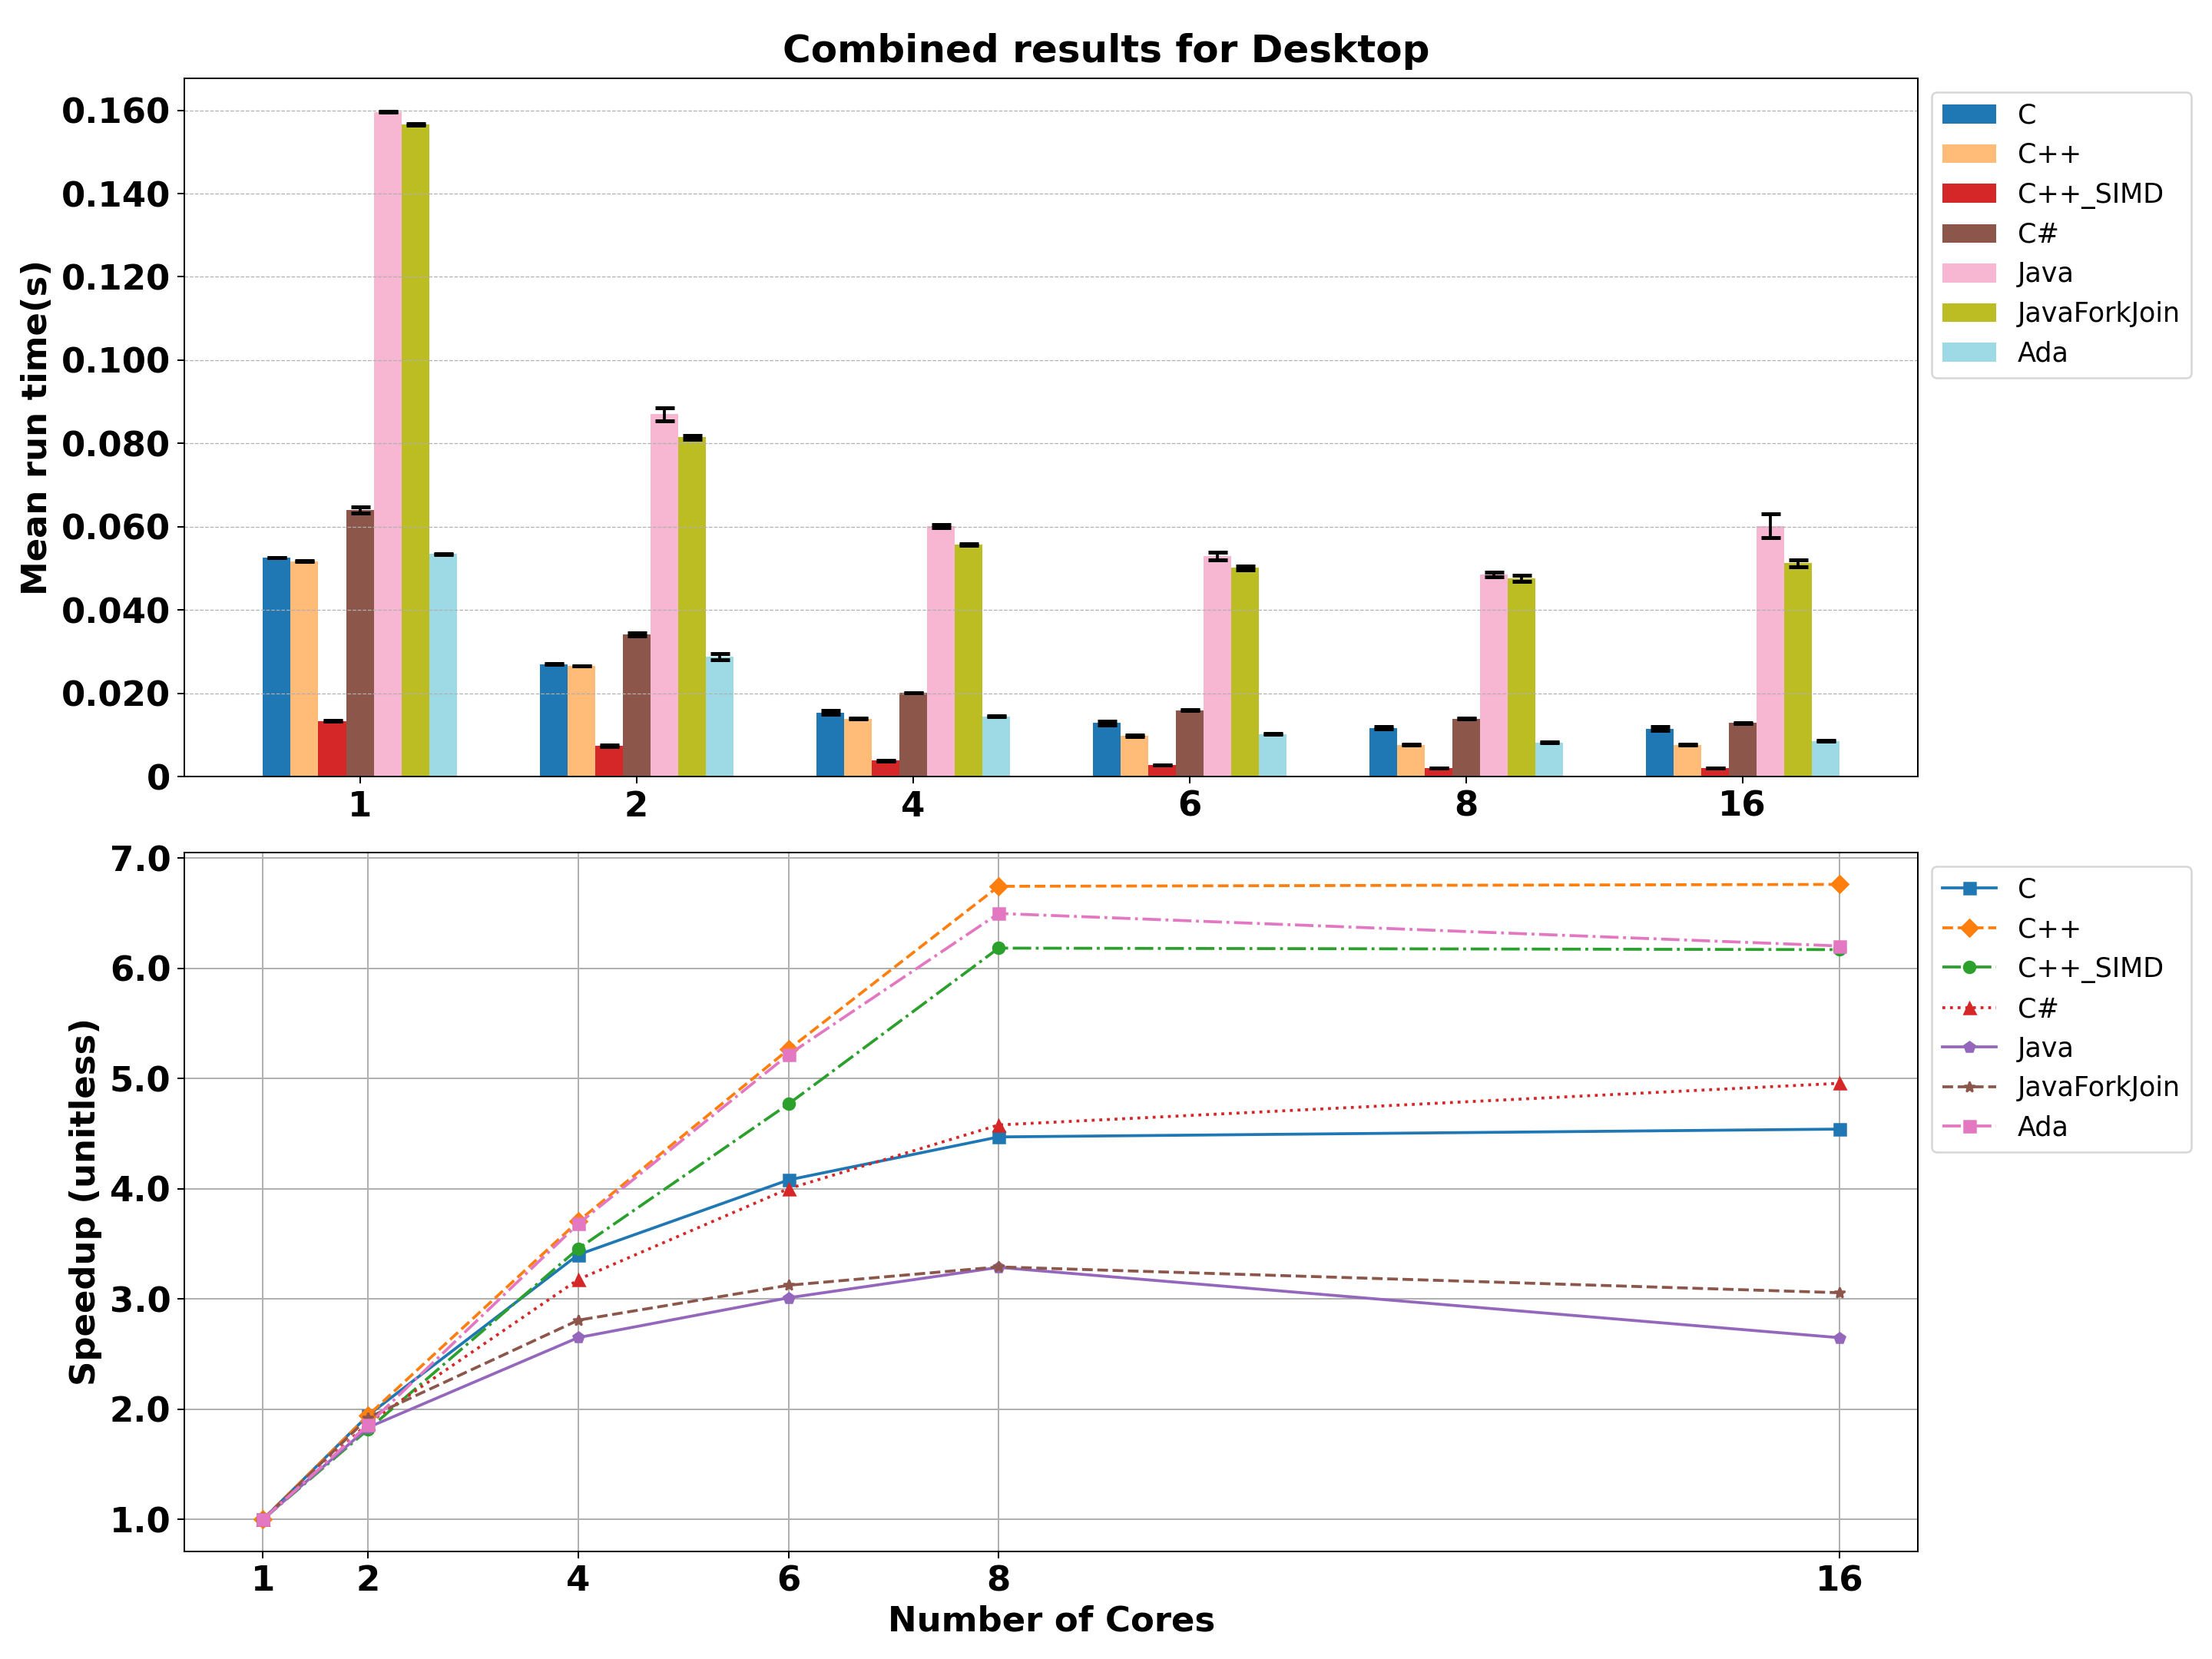
\includegraphics[width=1\textwidth, height=10cm]{~/Documents/Part_D_Modules/Individual_Project/Individual_report/figures/mpbenchmark_desktop_results.png} % Adjust the path and width as needed
	\caption{Mean benchmark plot in seconds shown top. Speedup plot shown bottom.}
	\label{fig:mpbenchmark_desktop_plot} % Use this label to reference the figure
\end{figure}


On desktop(\texttt{x86}) processor, \texttt{AVX2} instructions were used to implement SIMD intrinsics therefore, a comparison of decimal precision against the original unoptimised SIMD code is shown in Table ~\ref{tab:c++_avx2_pi} with run time collected using 16 cores. 

\begin{table}[htbp]
	\centering
	\begin{tabular}{ccc}
		\hline
		\textbf{Programming language/configuration} & \textbf{Decimal value of $\pi$} & \textbf{Mean run time(s)} \\ \hline
		\texttt{C++}             & 3.1415926535897643 &  0.007659 \\ \hline
		\texttt{C++/AVX2}   & 3.1415926535899033 &  0.002173  \\ \hline
		\texttt{C}                 & 3.1415926535897643 & 0.011577 \\ \hline
		\texttt{Ada}             & 3.1415926535897643 &  0.008623\\ \hline
	\end{tabular}
	\label{tab:c++_avx2_pi}
	\caption{Comparing the decimal precision of the \texttt{AVX2} enhanced solution with the original.}
\end{table}

% Talk about C++ solution outperforming the original in both run times and speedup 
% C++ SIMD enhanced outperformed even more with a lower speedup.
% Talk about SMT's benefits if any
% Discuss AVX2's decimal precision

The proposed \texttt{C++} solution outperformed the original implementations in \texttt{C} and \texttt{Ada} by over 11\%, marking a significant reduction in runtime. Additionally, it achieved a higher speed-up compared to the \texttt{Ada} solution, as illustrated in Figure~\ref{fig:mpbenchmark_desktop_plot}. The SIMD-enhanced solution achieved a remarkable runtime reduction of over 70\%, significantly outperforming all other solutions. However, this version did not show as large a speedup when run with an increased number of threads, which is not surprising given the already low runtime with a single thread. Moreover, the \texttt{AVX2}-enhanced code demonstrated decimal precision up to 12 decimal places, with discrepancies appearing from the 13th decimal place onwards, as shown in Table~\ref{tab:c++_avx2_pi}. This suggests a slight consideration that using \texttt{AVX2} instructions might lead to reduced precision for calculations requiring high decimal accuracy. However, the reduction in decimal precision has been minor, and its effects on the application have been largely inconsequential. Given the dramatic improvement in performance with \texttt{AVX2} instructions, the minor loss of decimal precision seems negligible compared to the benefits. Both solutions have met their objectives, with the first achieving superior speed-up and the second providing insights into CPU performance when SIMD intrinsics are utilized.

Another noteworthy observation is the lack of performance gain when scaling from 8 to 16 cores. The processor used supports simultaneous multi-threading (SMT), commonly branded as ``Hyper-threading" for Intel CPUs, which is typical in modern \texttt{x86} processors. SMT theoretically allows each physical core to execute two threads, and an 8-core processor with SMT would appear to have 16 cores. However, the proposed solutions, along with other compiled languages like \texttt{C} and \texttt{Ada}, showed negligible performance gains by utilizing the virtual cores. \texttt{Java} experienced a slight performance degradation, while \texttt{C\#} was the only language to demonstrate a performance increase. Using the results from the \texttt{x86} processor, we can conclude that the additional cores provided by SMT did not enhance performance and, in some cases, even degraded it.

Figures ~\ref{fig:mpbenchmark_rpi5_plot} and ~\ref{fig:mpbenchmark_rpi4_plot} show the results collected from the latest Raspberry Pi 5 (\texttt{Cortex A-76} processor) and Raspberry Pi 4(\texttt{Cortex A-72} processor) respectively.

\begin{figure}[htbp] % Positioning preference: here, top, bottom, page
	\centering
	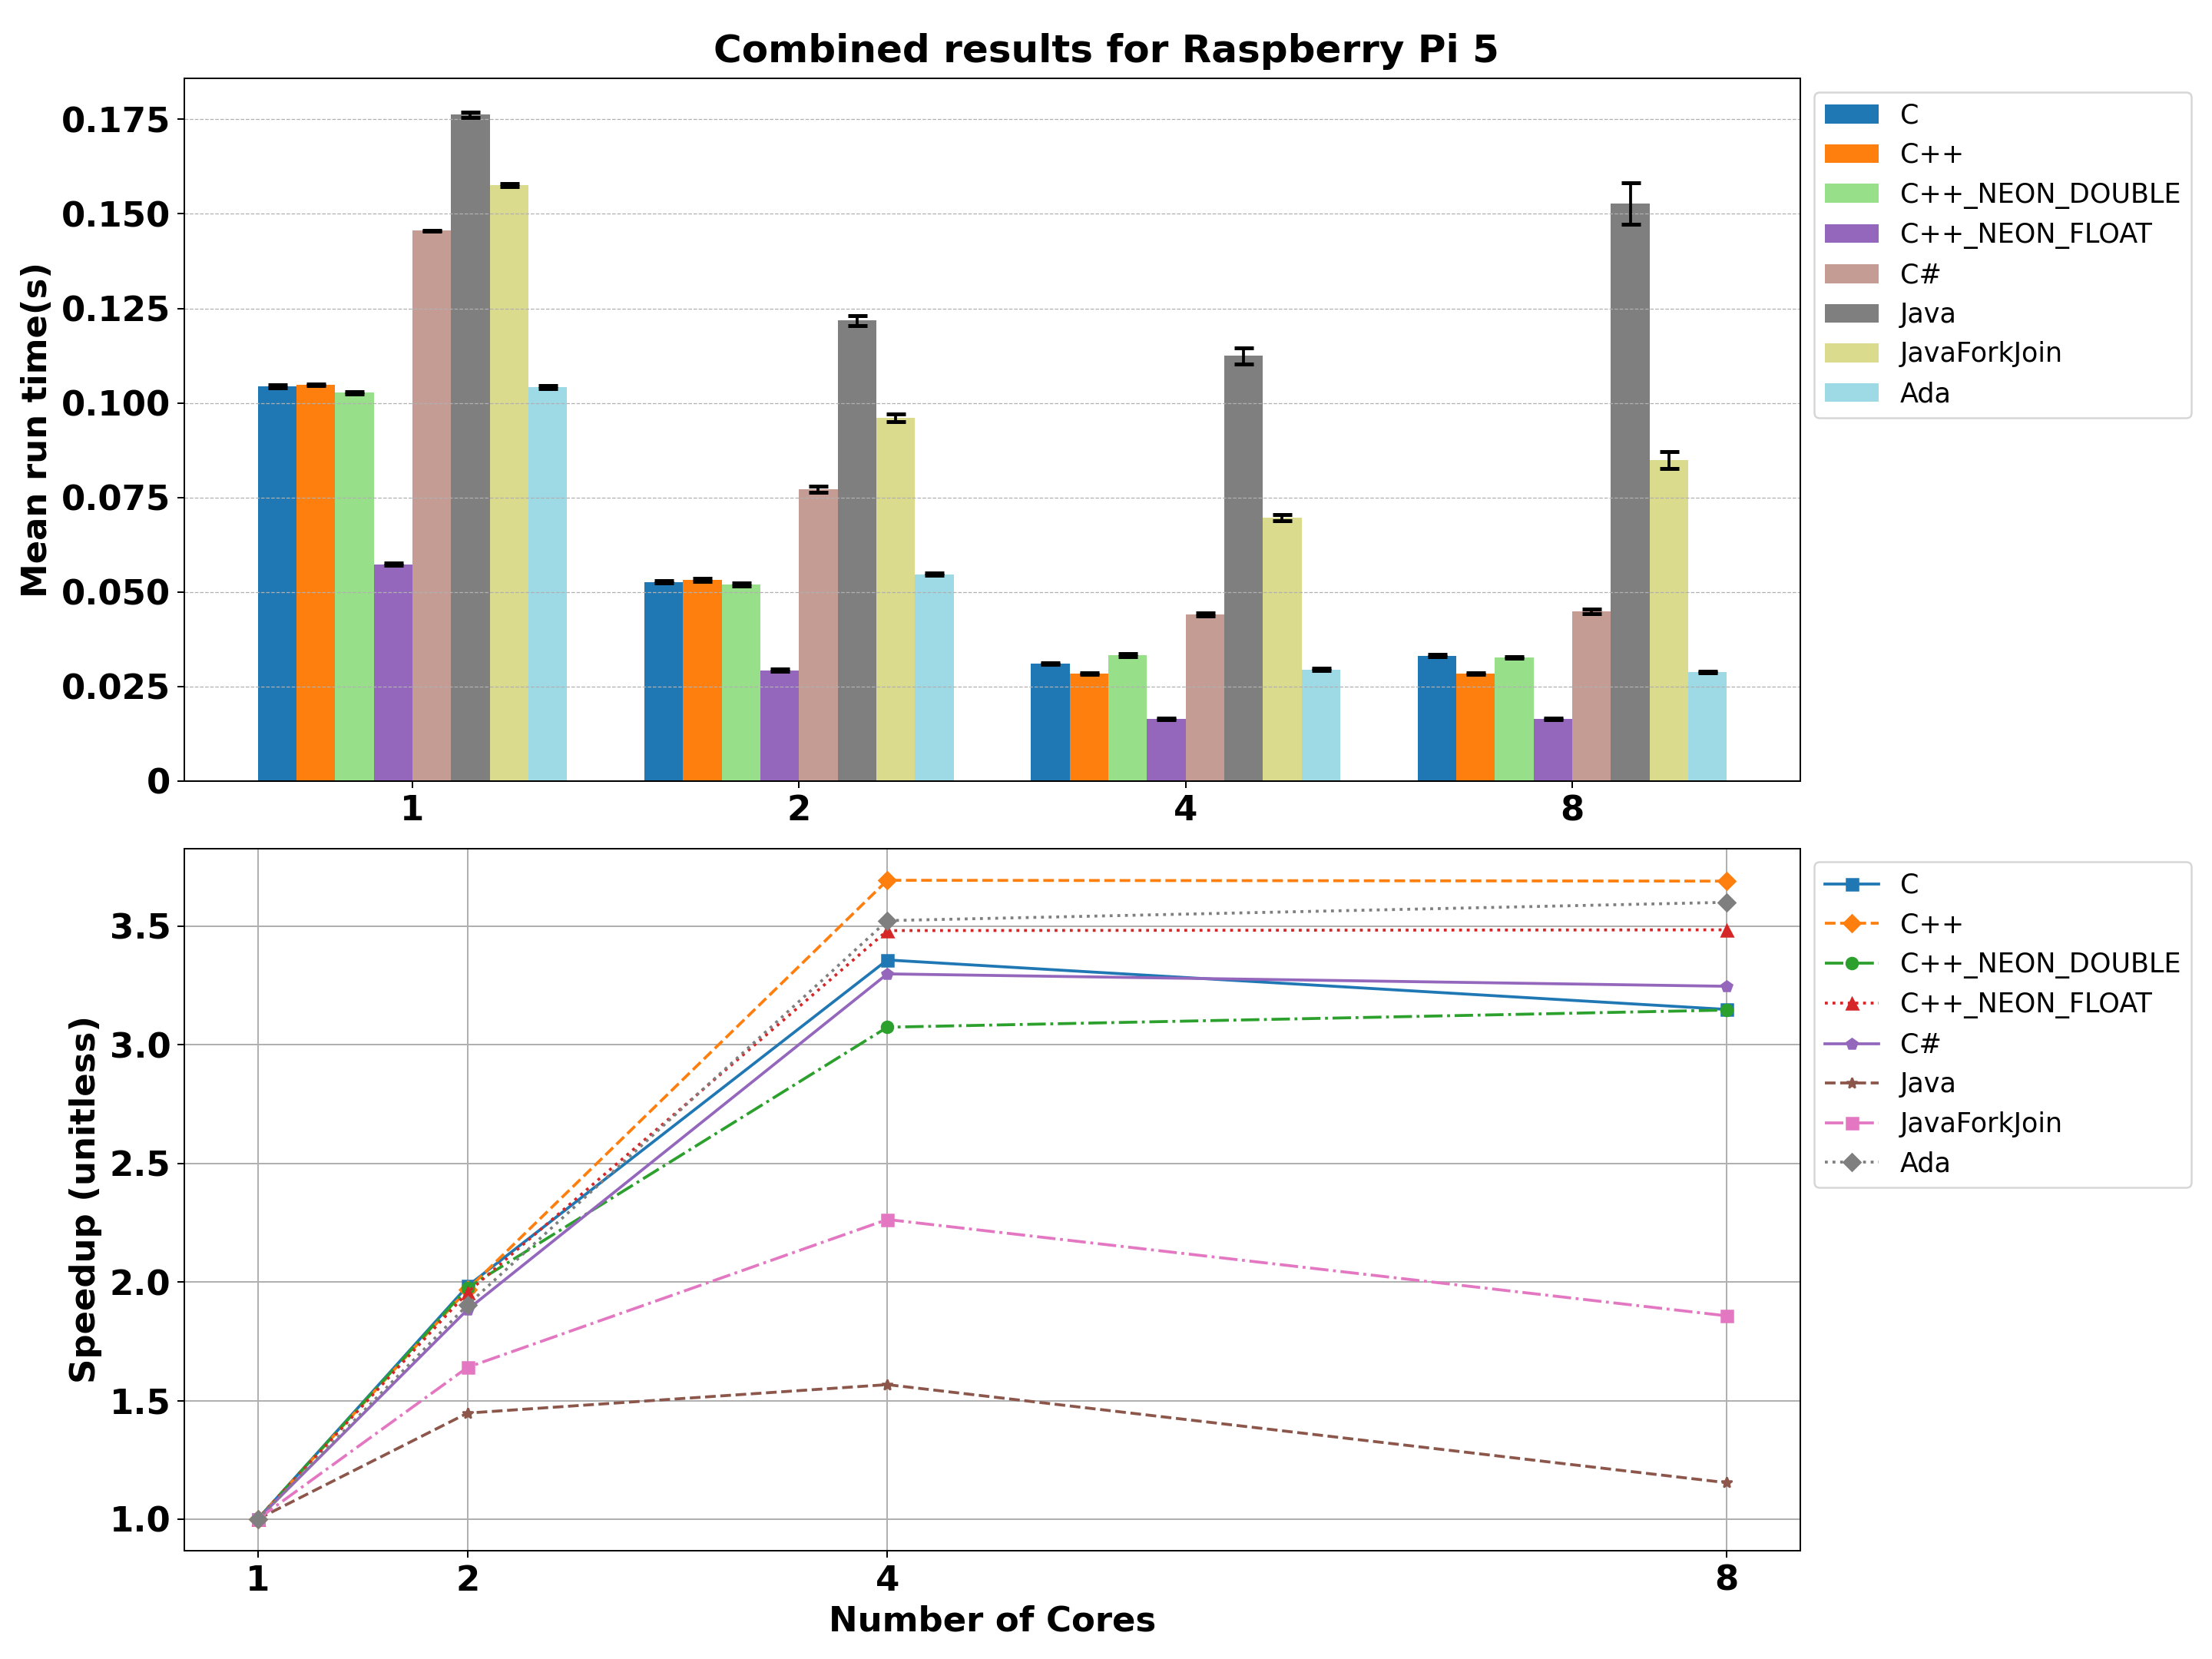
\includegraphics[width=1\textwidth, height=10cm]{~/Documents/Part_D_Modules/Individual_Project/Individual_report/figures/mpbenchmark_rpi5_results2.png} % Adjust the path and width as needed
	\caption{Mean benchmark plot in seconds shown top. Speedup plot shown bottom.}
	\label{fig:mpbenchmark_rpi5_plot} % Use this label to reference the figure
\end{figure}

\begin{figure}[htbp] % Positioning preference: here, top, bottom, page
	\centering
	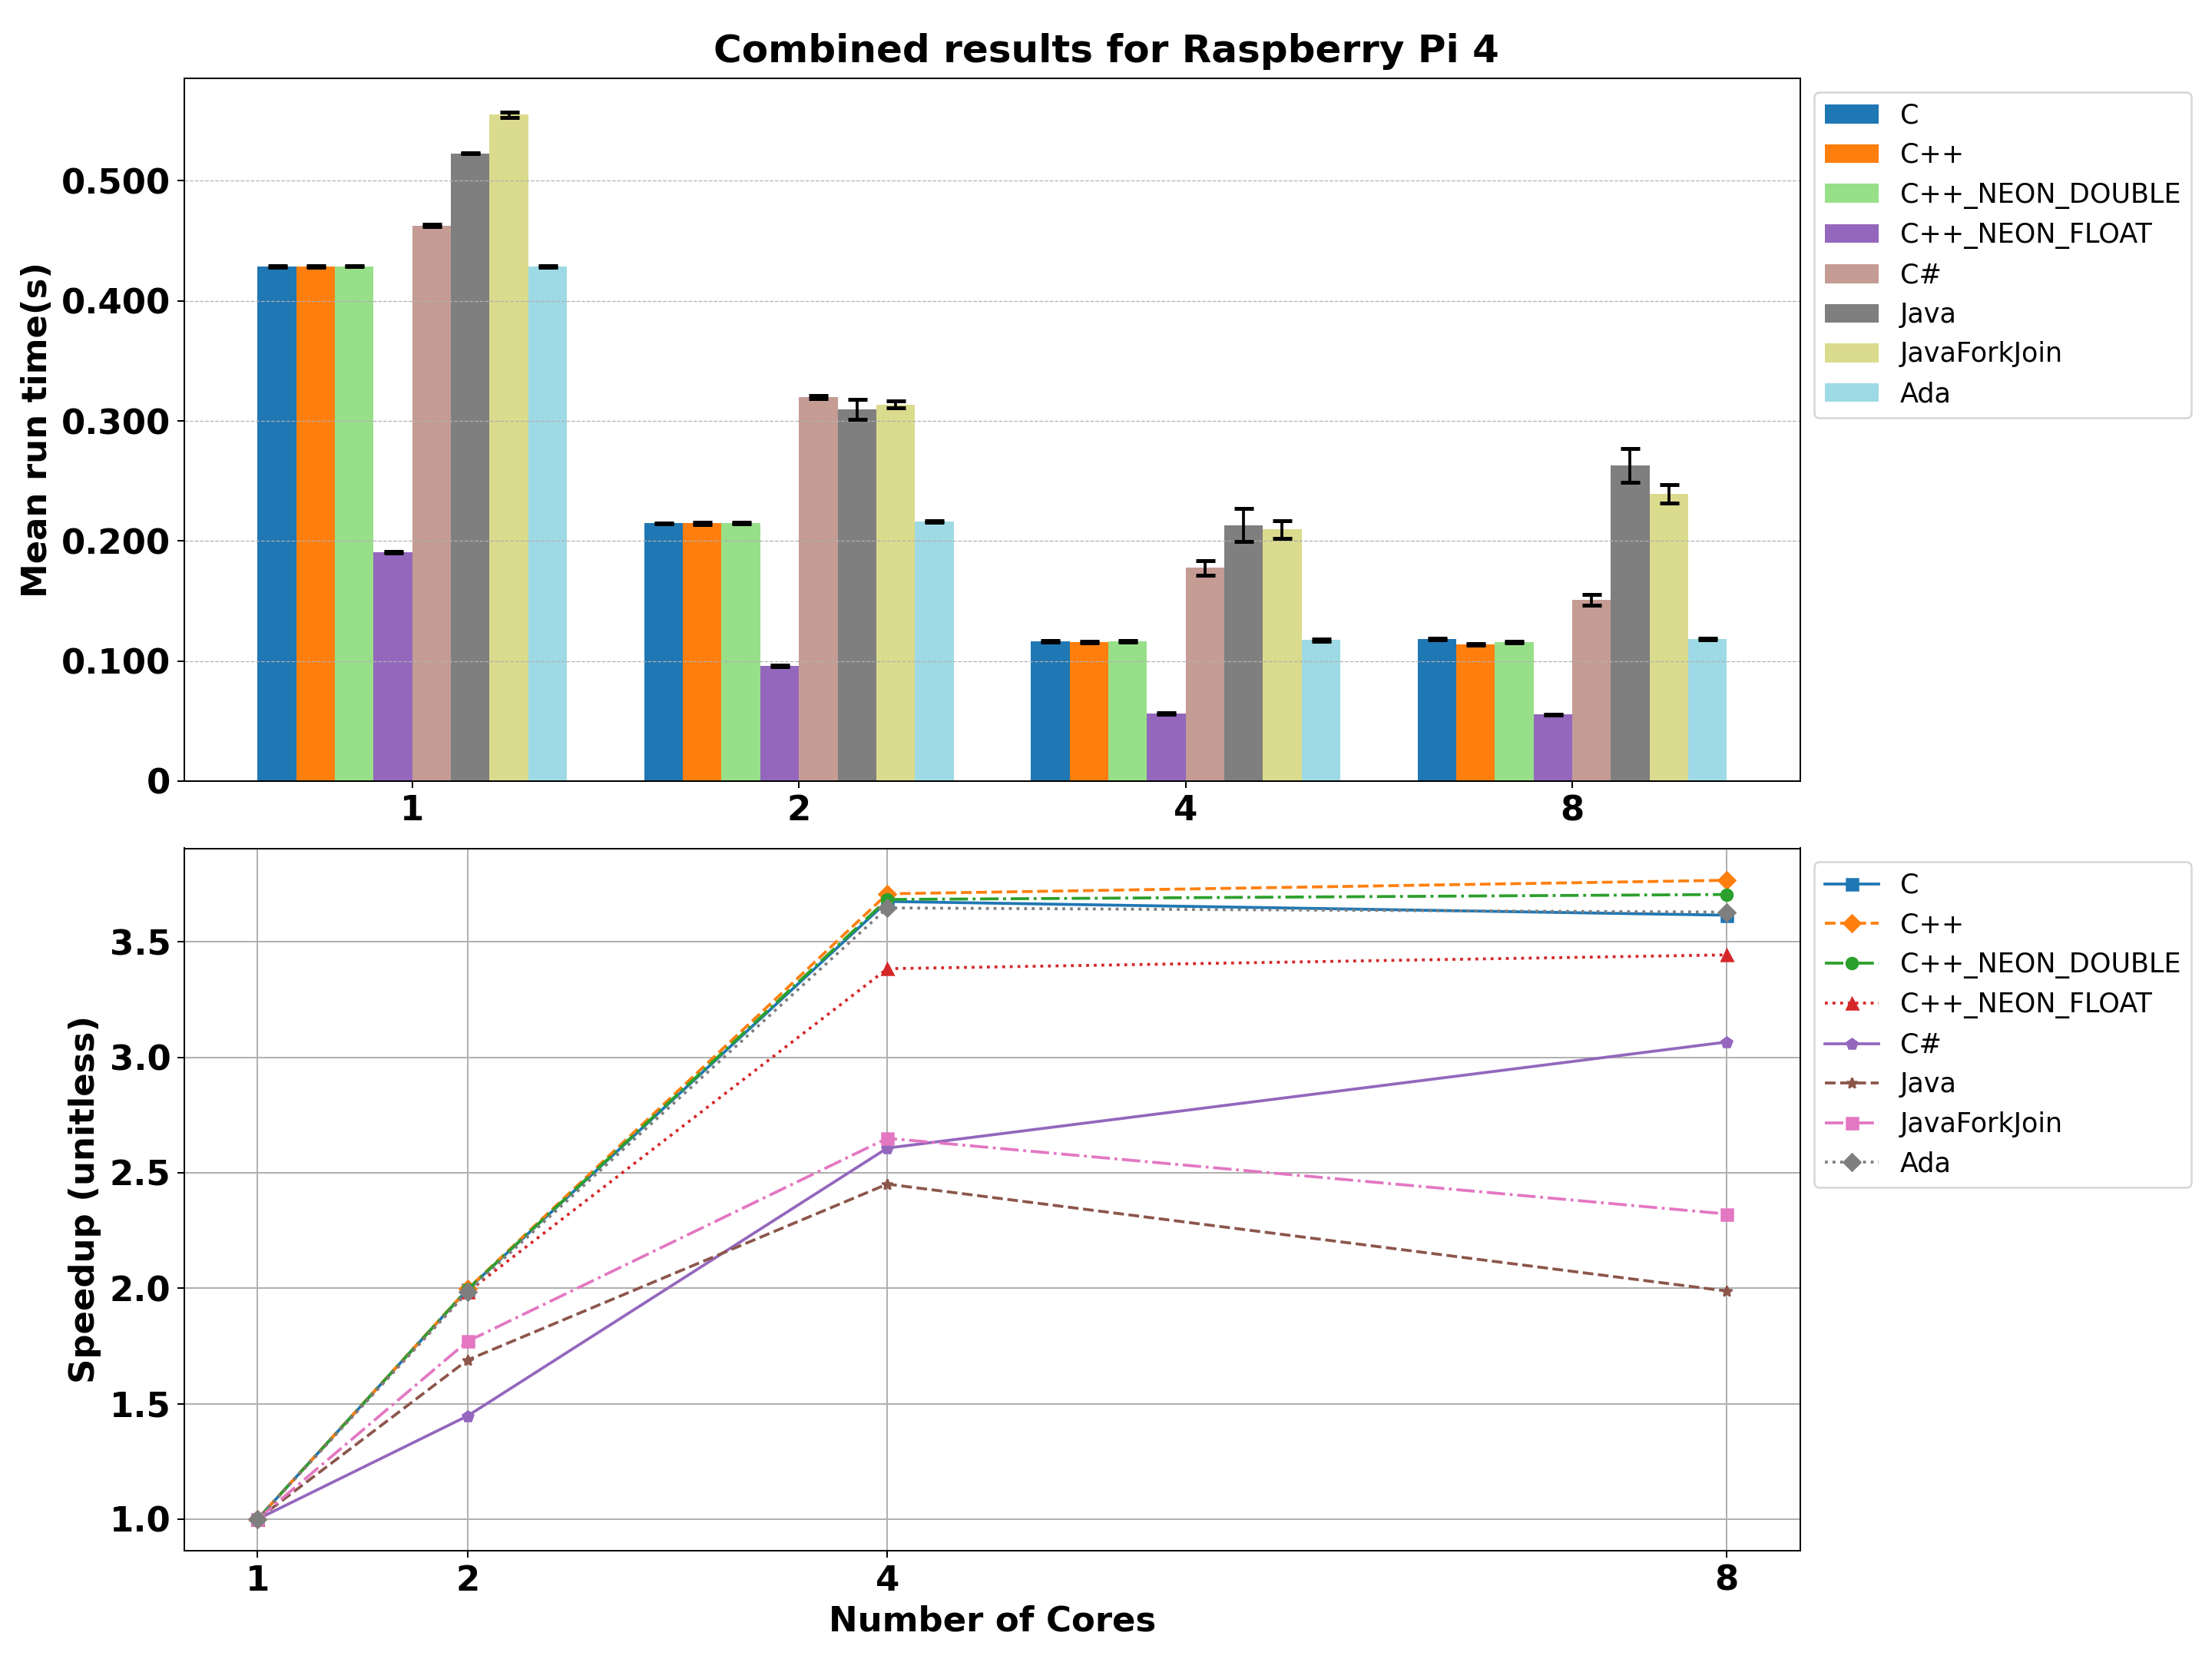
\includegraphics[width=1\textwidth, height=10cm]{~/Documents/Part_D_Modules/Individual_Project/Individual_report/figures/mpbenchmark_rpi4_results2.png} % Adjust the path and width as needed
	\caption{Mean benchmark plot in seconds shown top. Speedup plot shown bottom.}
	\label{fig:mpbenchmark_rpi4_plot} % Use this label to reference the figure
\end{figure}

The decimal precision of using single and double precision floating point \texttt{NEON} instructions on the Raspberry Pi processors is compared in Table ~\ref{tab:c++_neon_pi}, with run time collected using 4 cores. 

\begin{table}[htbp]
	\centering
	\begin{tabular}{cccc}
		\hline
		\textbf{Programming language/configuration} & \textbf{Decimal value of $\pi$} & \textbf{Run time RPI5(s)} & \textbf{Run time RPI4(s)} \\ \hline
		\texttt{C++}                                                   & 3.1415926535897643 & 0.028356  & 0.115569 \\ \hline
		\texttt{C++/single-precision NEON}              & 3.141531467437744   &  0.016477 & 0.056352 \\ \hline
		\texttt{C++/double-precision NEON}             & 3.14159265358986     & 0.033399  & 0.116423 \\ \hline
		\texttt{C}                                                        & 3.1415926535897643 & 0.031107  & 0.116538\\ \hline 
		\texttt{Ada}                                                    & 3.1415926535897643  & 0.029549  & 0.117536 \\ \hline
	\end{tabular}
	\label{tab:c++_neon_pi}
	\caption{Comparing the decimal precision of the \texttt{NEON} enhanced solutions.}
\end{table}

% Talk about the proposed solution's performance in PI5 and PI4. 
% Talk about the speedup
% Talk about NEON solutions and their respective decimal precision.
% Can include the comparision with other solutions in the appendix, like Java and C# and Raspberry Pi 3 

The proposed solution outperformed both the \texttt{C} and \texttt{Ada} solutions in terms of runtime and speedup. On the Raspberry Pi 5, a slight reduction in runtime (about 4\%) and a notable improvement in speedup were observed. The results on the Raspberry Pi 4 were less impressive, showing only a 1\% improvement in performance and a marginal increase in speedup. Nevertheless, the proposed \texttt{C++} solution outperformed the original solutions in terms of runtime and speedup on both Raspberry Pi devices, although the improvement was marginal on the Raspberry Pi 4.

The \texttt{NEON} enhanced solutions using single precision floating-point produced over a 40\% reduction in run time at the cost of lower speedup across threads and a reduced decimal precision to four decimal places. On the Raspberry Pi 5, the \texttt{NEON} solution using double precision failed to reduce runtime and produced the worst overall speedup across varying numbers of threads. On the Raspberry Pi 4, the \texttt{NEON} double precision solution did not reduce the runtime and produced a similar speedup to other solutions. However, the double precision solutions did offer far superior decimal precision, up to 12 decimal places. Given \texttt{NEON} instructions' reduced support for double precision floating points, developers must choose between single precision for significantly improved performance but lower decimal precision, and double precision, which did not improve performance on the tested embedded processors. These results are summarised in Table~\ref{tab:c++_neon_pi}. When comparing ``deadlines missed", on desktop and Raspberry Pi 5 there were no ``deadlines missed" from any of the compiled languages. On Raspberry Pi 4, the proposed \texttt{C++} solution missed a few deadlines reporting a noticeable improvement over \texttt{C} and \texttt{Ada} versions however the \texttt{NEON} single solution did not miss any deadlines showcasing a great improvement not just in run time but also in the ``deadline missed" category. In depth results about ``deadlines missed" and results from Raspberry Pi 3 were slightly tangential to the project's main objective, therefore they can be found in the [Appendix ~\ref{sec:app_obj1}].

Benchmarks allow us to compare the latest Raspberry Pi 5 (\texttt{Cortex A-76}) against the older Raspberry Pi 4 (\texttt{Cortex A-72}). The \texttt{Cortex A-76} performed 75\% faster in terms of runtime when comparing the proposed \texttt{C++} solution, roughly \texttt{4x} faster. The \texttt{Cortex A-76} processor offered a 42\% reduction in runtime when \texttt{NEON(float)} enhanced code was used compared to a 51\% reduction in runtime for the \texttt{Cortex A-72}. Both processors exhibited a lower speedup when \texttt{NEON} instructions were used, similar to what was observed with the \texttt{x86} processor. The superior performance of the \texttt{Cortex A-76} may be attributed to a faster clock speed of 2.4 GHz compared to 1.5GHz of the older \texttt{Cortex A-72} \cite{rasp_pi5_pi4_comparision}.

The proposed \texttt{C++} solution surpassed the previously developed \texttt{mpbenchmark}\cite{mpbenchmark_paper} on both \texttt{x86} and \texttt{ARM} processors. It offered better speedup across threads, and an alternate novel \texttt{SIMD} enhanced version (where the application decides whether to use \texttt{AVX2} or \texttt{NEON} depending on the processor type) can be utilised to analyse the CPUs' SIMD performance and scalability. This unprecedented improvement is part of an upcoming publication.

\section{Objective 2: \texttt{MobileNet}}

Figure ~\ref{fig:mobilenet_desktop_plot} shows the results collected after parallelising \texttt{MobileNet}, from desktop(\texttt{x86} processor). The results show a comparison between SIMD optimisations turned on or off. 

\begin{figure}[htbp] % Positioning preference: here, top, bottom, page
	\centering
	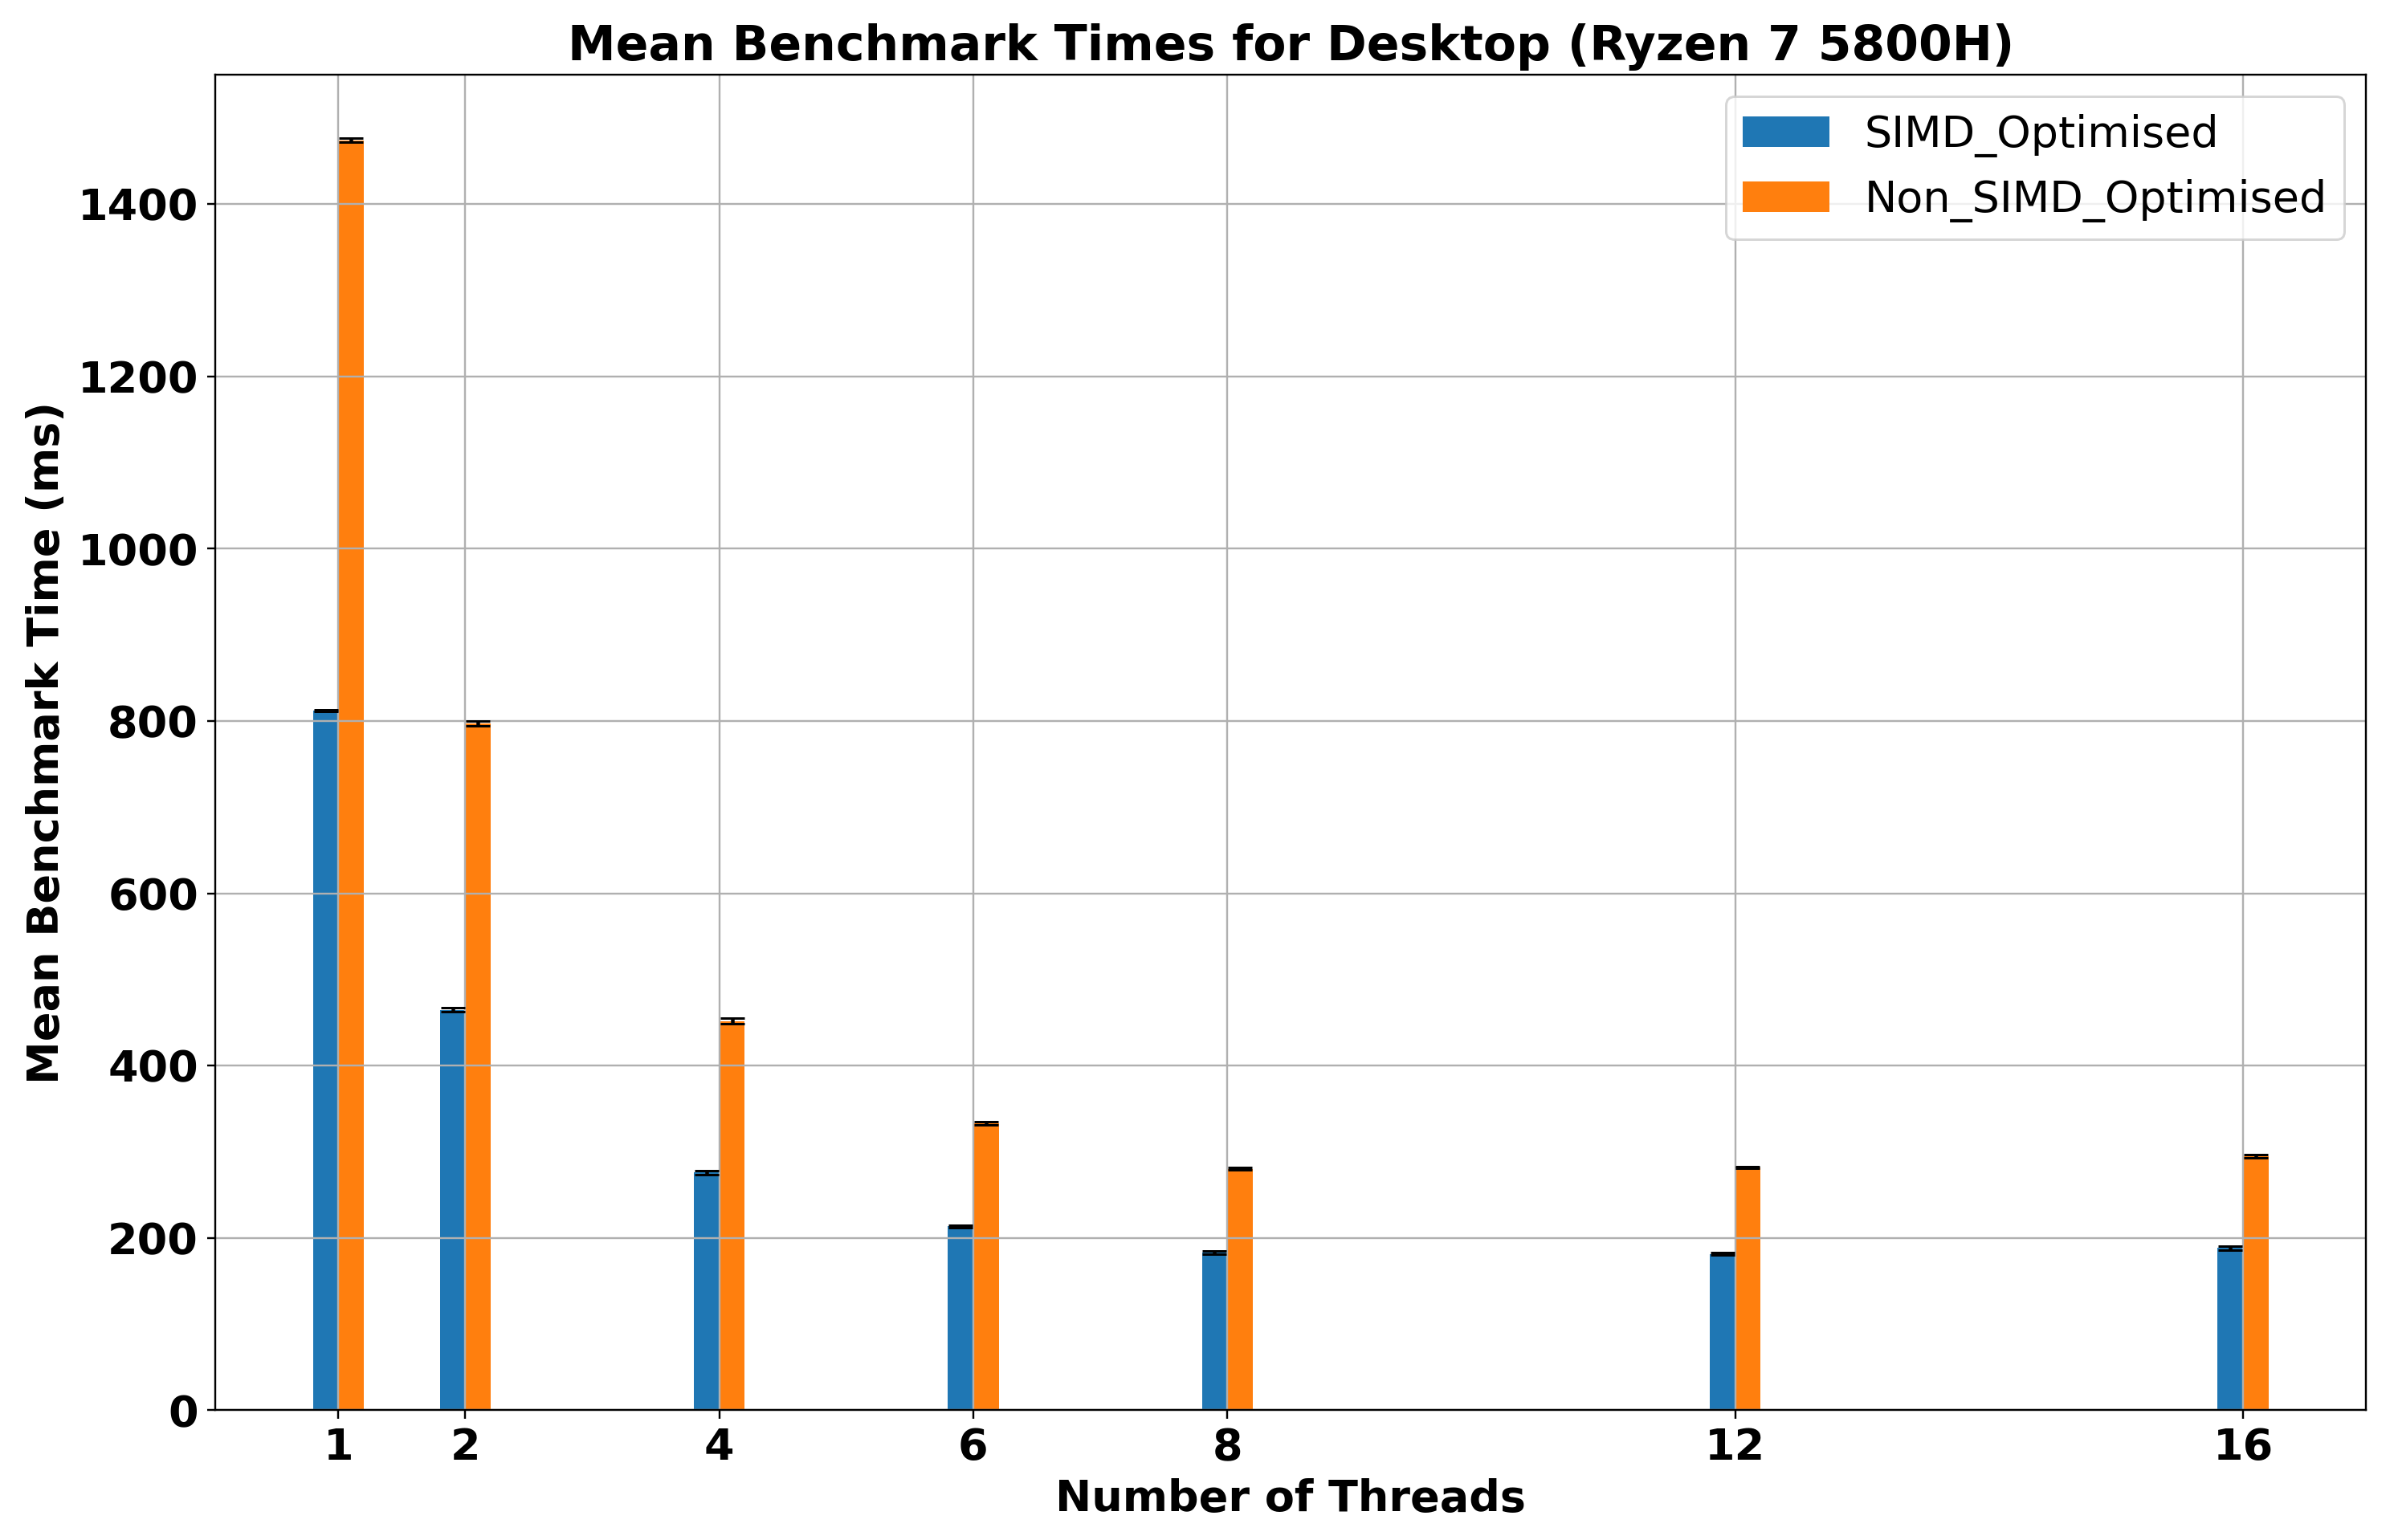
\includegraphics[width=1\textwidth, height=10cm]{~/Documents/Part_D_Modules/Individual_Project/Individual_report/figures/mobilenet_desktop.png} % Adjust the path and width as needed
	\caption{Mean benchmark plot in milliseconds shown top. Speedup plot shown bottom.}
	\label{fig:mobilenet_desktop_plot} % Use this label to reference the figure
\end{figure}

The mean benchmark time of the original \texttt{MobileNet} application\cite{mobilenet_repo} was 1474.2 ms(using the \texttt{-O3} optimisation flag). The benchmark time using the maximum threads(16) with SIMD was 188.24ms and without SIMD it was 294.68ms. The SIMD optimisations were turned on and off as shown in Listing  ~\ref{lst:mobilenet_parallel}. This presents a drastic reduction in run time of 87.2\% and 80.0\% for the SIMD and non-SIMD solutions respectively. Using multi-threading on the desktop processor yielded exceptional results and a dramatic improvement of the application. The results also indicate a performance degradation when using threads greater than 8 which is the maximum physical cores on the system. Both of the solutions produced a slight degradation of performance when going from 8 to 16 threads, suggesting once again the virtual cores from SMT did not yield in performance gains. 

The performance on the Raspberry Pi devices was a little more nuanced. The results of having different parallel regions and SIMD optimisations turned on or off were compared. The plots have the following legends:

\begin{enumerate}
	\item \texttt{\seqsplit{3\_Parallel\_Regions\_SIMD}}: all three functions \texttt{\seqsplit{ConvLayer::forward()}}, \texttt{\seqsplit{BatchNormalLayer::forward()}} and \texttt{\seqsplit{ConvLayer::Addpad()}} have been parallelised with SIMD optimisations.
	\item \texttt{\seqsplit{3\_Parallel\_Regions}}: all three functions \texttt{\seqsplit{ConvLayer::forward()}}, \texttt{\seqsplit{BatchNormalLayer::forward()}} and \texttt{\seqsplit{ConvLayer::Addpad()}} have been parallelised without SIMD optimisations.
	\item \texttt{\seqsplit{2\_Parallel\_Regions\_SIMD}}: only two functions \texttt{\seqsplit{ConvLayer::forward()}} and \texttt{\seqsplit{BatchNormalLayer::forward()}} have been parallelised with SIMD optimisations.
	\item \texttt{\seqsplit{2\_Parallel\_Regions}}: only two functions \texttt{\seqsplit{ConvLayer::forward()}} and \texttt{\seqsplit{BatchNormalLayer::forward()}} have been parallelised without SIMD optimisations.
\end{enumerate}

Figures ~\ref{fig:mobilenet_rpi5_plot} and ~\ref{fig:mobilenet_rpi4_plot} show results collected from Raspberry Pi 5 and Raspberry Pi 4 respectively. 

\begin{figure}[htbp] % Positioning preference: here, top, bottom, page
	\centering
	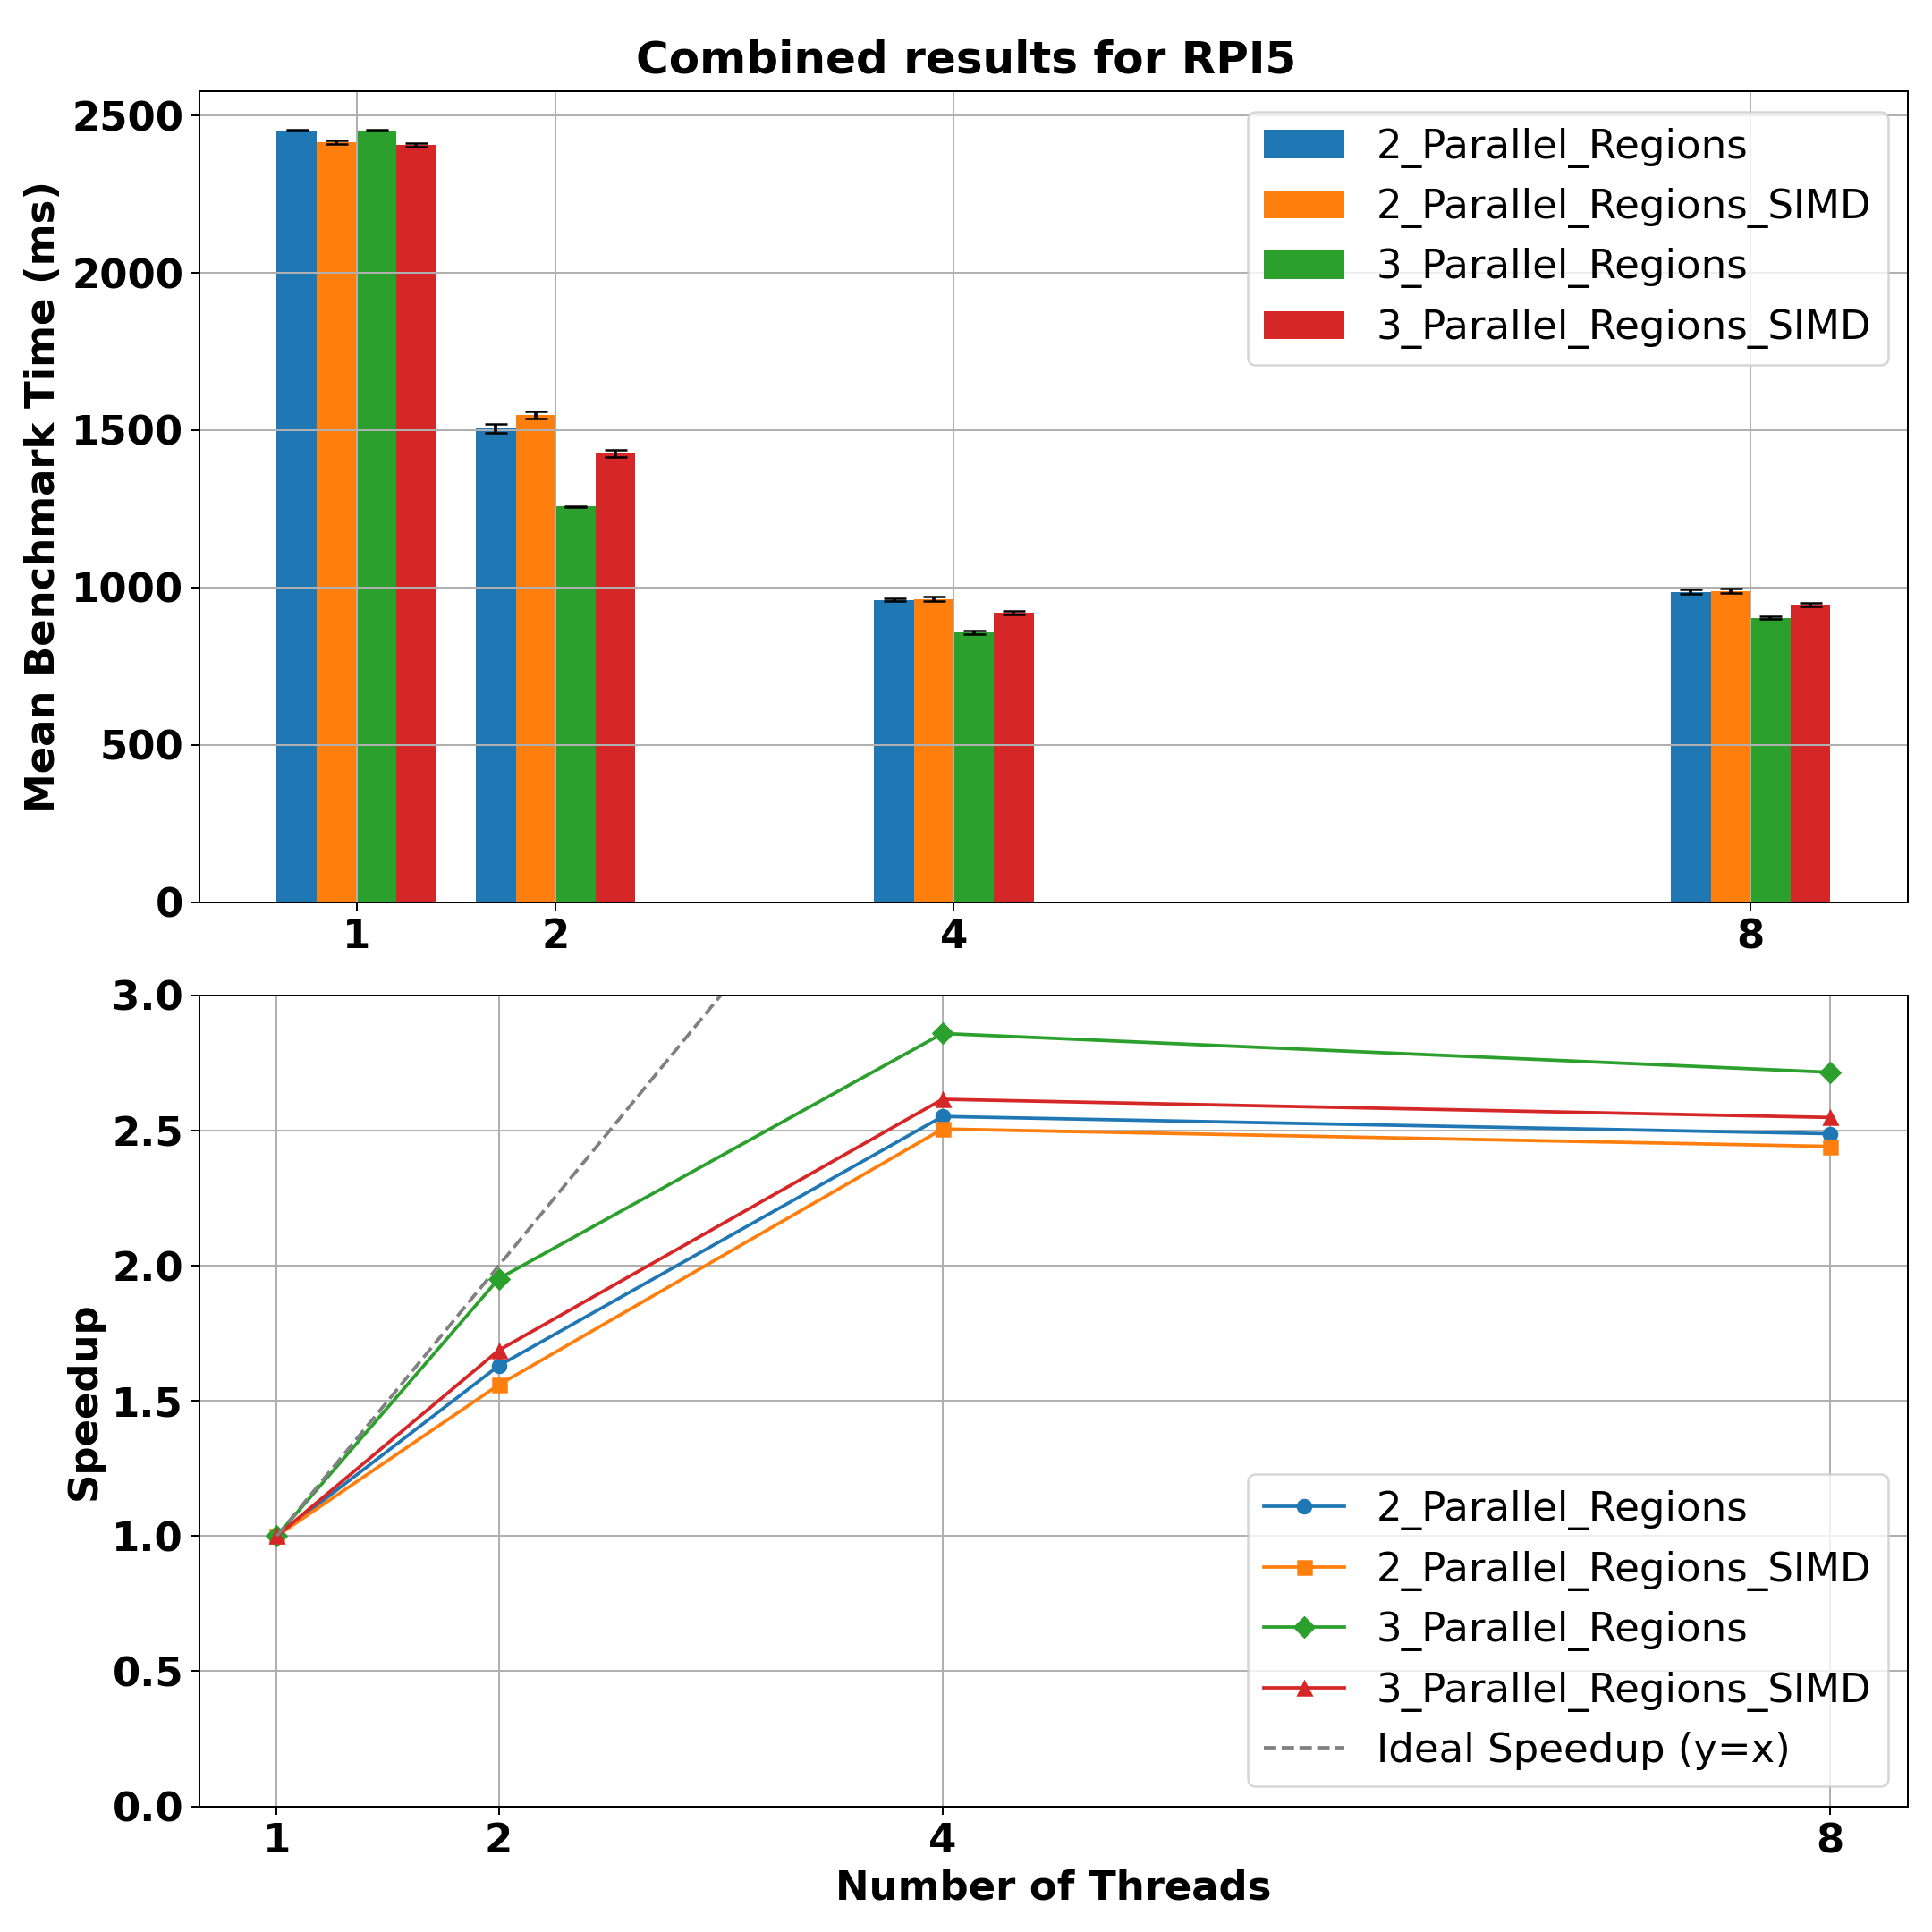
\includegraphics[width=1\textwidth, height=10cm]{~/Documents/Part_D_Modules/Individual_Project/Individual_report/figures/mobilenet_rpi5.png} % Adjust the path and width as needed
	\caption{Mean benchmark plot in milliseconds shown top. Speedup plot shown bottom.}
	\label{fig:mobilenet_rpi5_plot} % Use this label to reference the figure
\end{figure}

\begin{figure}[htbp] % Positioning preference: here, top, bottom, page
	\centering
	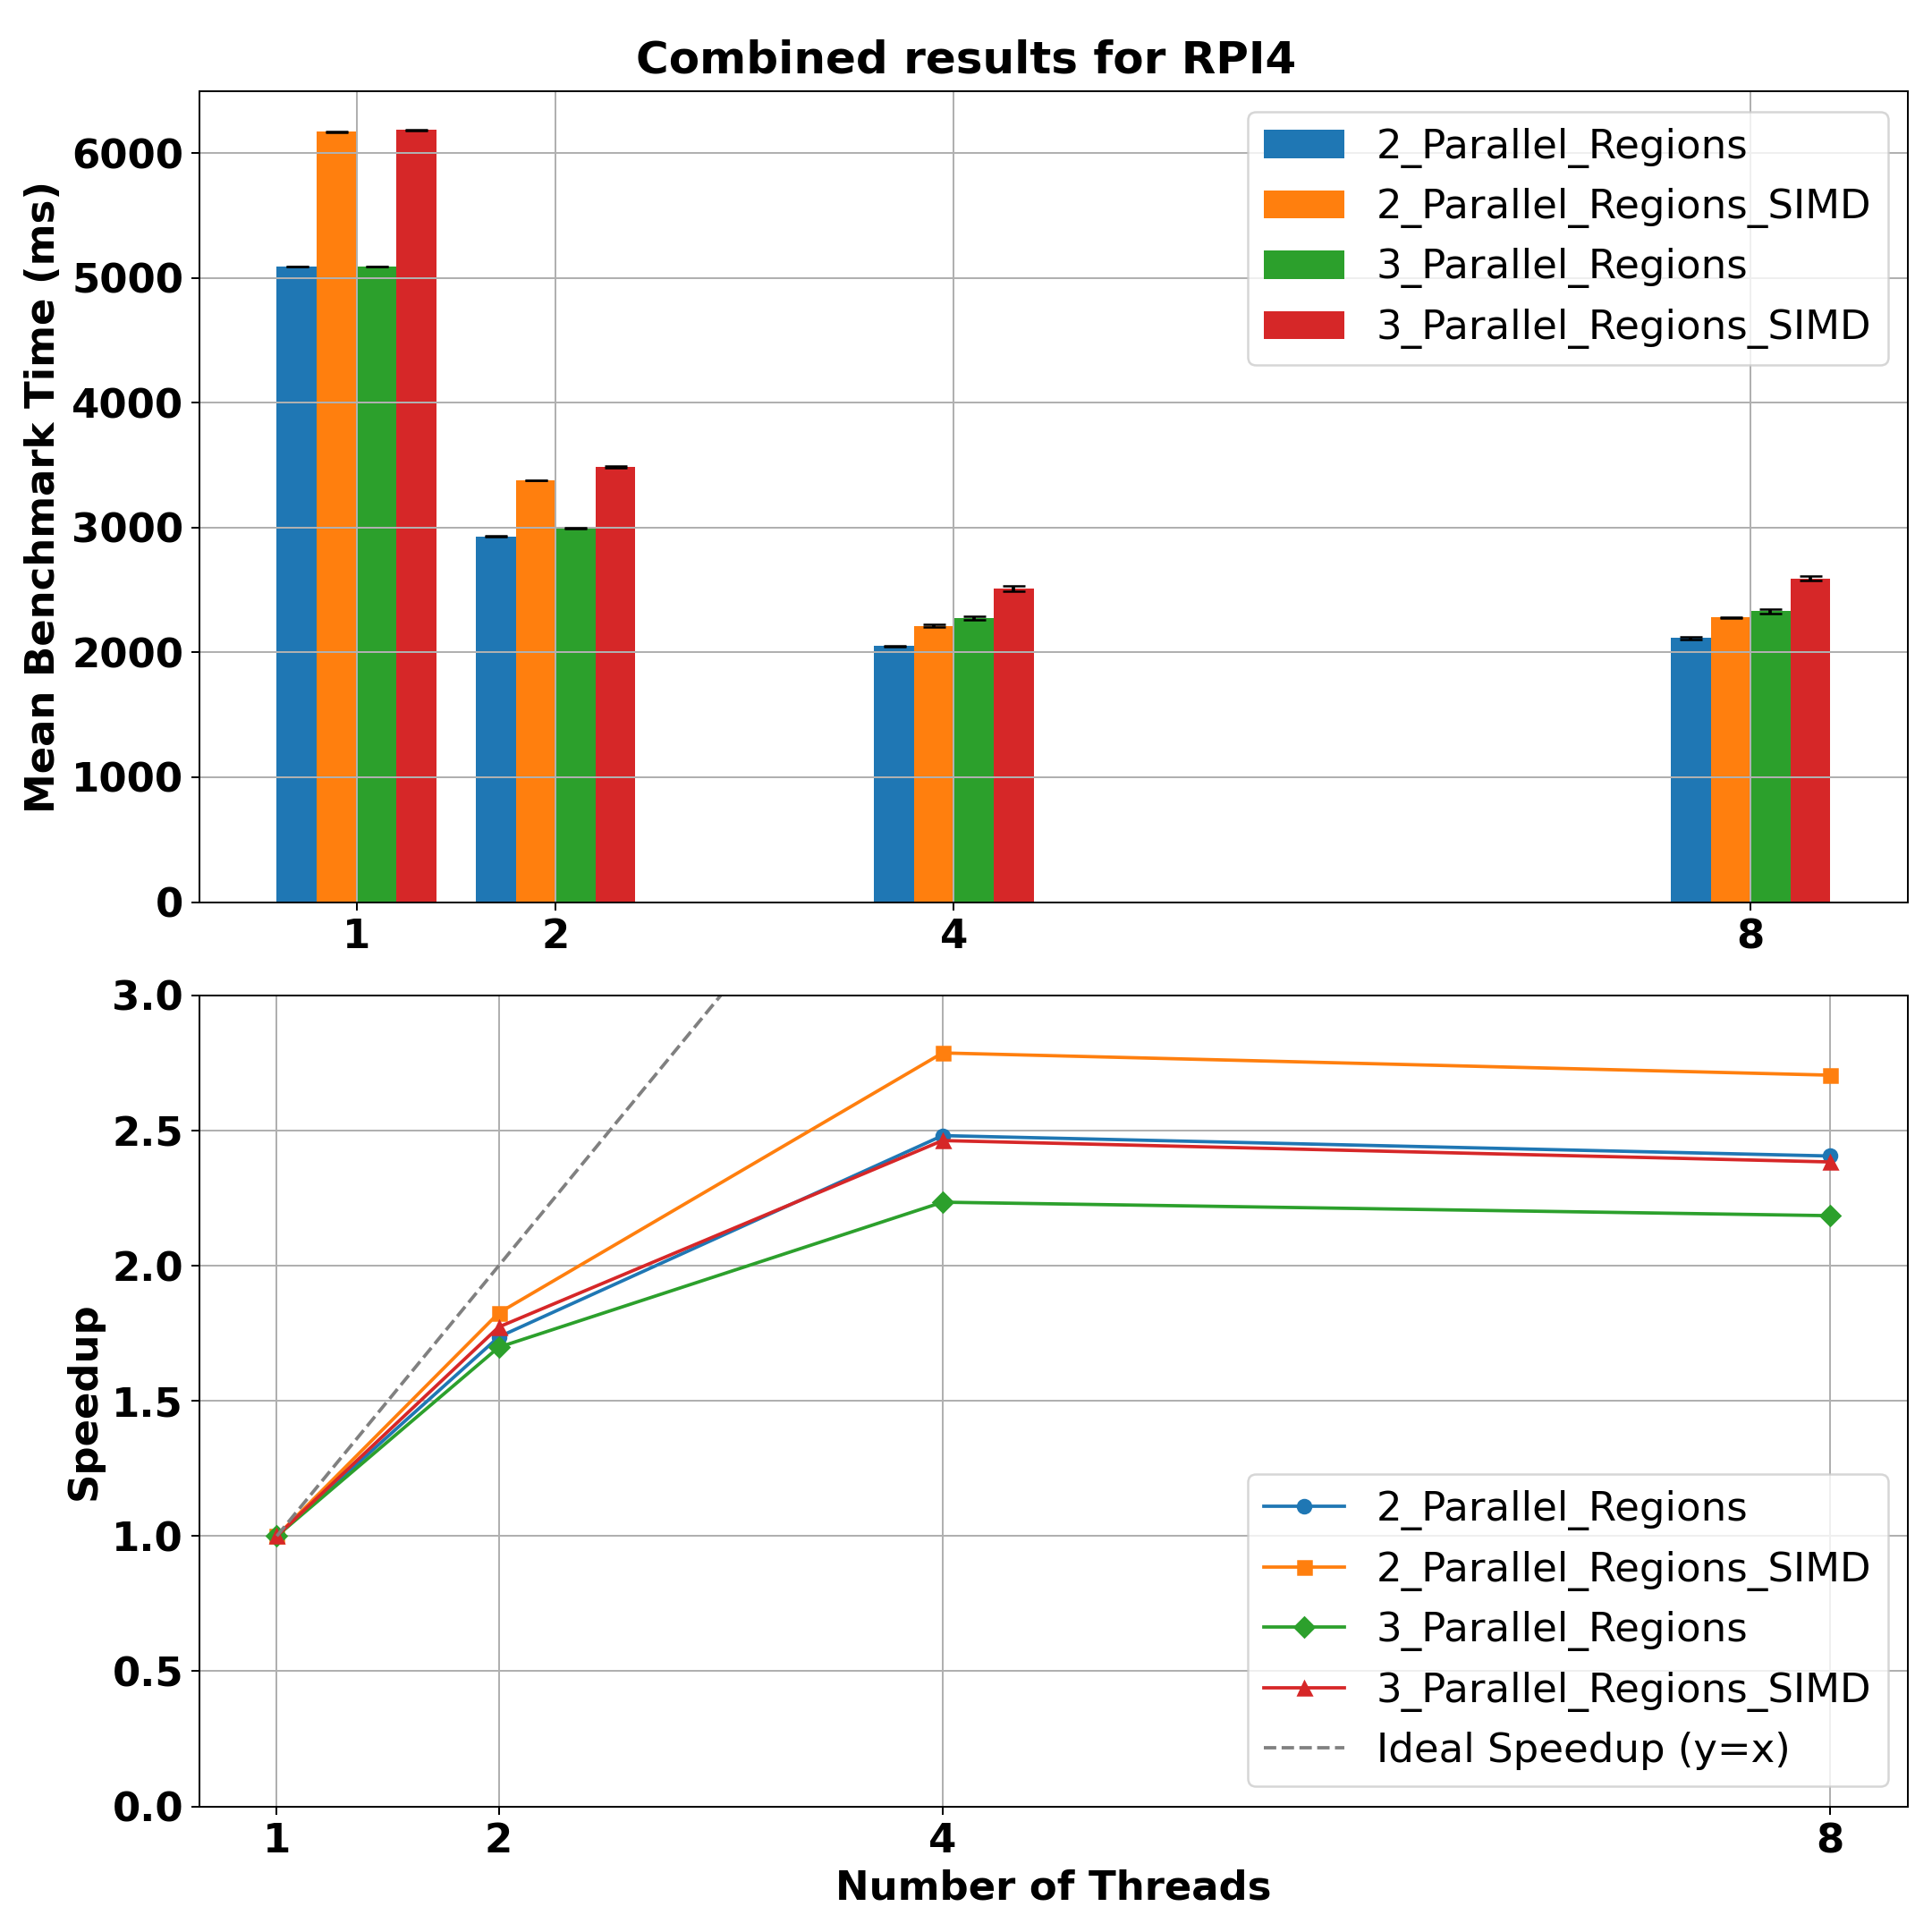
\includegraphics[width=1\textwidth, height=10cm]{~/Documents/Part_D_Modules/Individual_Project/Individual_report/figures/mobilenet_rpi4.png} % Adjust the path and width as needed
	\caption{Mean benchmark plot in milliseconds shown top. Speedup plot shown bottom.}
	\label{fig:mobilenet_rpi4_plot} % Use this label to reference the figure
\end{figure}

\begin{table}[htbp]
	\centering
	\begin{tabular}{@{}lccc@{}}
		\toprule
		\textbf{Metric} & \textbf{Desktop} & \textbf{RPI5} & \textbf{RPI4} \\ \midrule
		% Row 1
		Original run time(ms)&1474.2&2462.33 &5108.77 \\ \hline
		% Row 2
		Lowest run time(ms)&188.24 &858.10 &2050.78 \\ \hline
		% Row 3
		Best speedup&5.26 &2.86 &2.79 \\ \hline
		% Row 4
		Optimal threads&8 &4 & 4\\ \hline
		% Row 5
		Performance gain versus original(\%)&87.2&65.2 & 59.90\\ \hline
		% Row 6
		Performance gain versus RPI4(\%)&90.8 &58.2 &0 \\
		\bottomrule
	\end{tabular}
	\caption{Comparing performance metrics across CPUs.}
	\label{tab:performance_comparison}
\end{table}

The results indicate that the optimal configuration for the Raspberry Pi 5 is ``\texttt{3\_Parallel\_Regions}". This resulted in the lowest run time and best overall speedup when compared to other configurations. For the Raspberry Pi 4 the results were harder to interpret, the lowest run time was achieved with ``\texttt{2\_Parallel\_Regions}" but the best speedup was achieved with ``\texttt{2\_Parallel\_Regions\_SIMD}". Surprisingly SIMD optimisations on both of the Raspberry Pi devices did not result in reduction of run time contrary to what was observed in objective 1. When comparing the two processors the \texttt{Cortex A-76} performed 58\% faster and offered the best performance with three parallel regions and also achieved a slightly better speedup(\texttt{2.86} versus \texttt{2.76}). Summarised results can be found in Table ~\ref{tab:performance_comparison}. These results indicate that the \texttt{Cortex A-76} is better able to take advantage of parallelised regions compared to the \texttt{Cortex A-72}.  

Contrasting to the Raspberry Pi devices the best performance on desktop was achieved with 3 parallel regions and SIMD optimisations. This presents an interesting challenge to the developer when porting this application on embedded devices, results collected from the Raspberry Pi devices showcase the need for tailoring the multi-threading architecture according to the target CPU to achieve optimal performance. Strangely the SIMD optimisations from the \texttt{OpenMP} library did not improve performance on the Raspberry Pi devices, this can be further investigated by manually implementing \texttt{NEON} instructions and compare its effects, similar to the method in objective 1. Both of the Raspberry Pi devices required slightly different configurations to achieve optimal performance. Optimal performance would be crucial in embedded processors part of drones and/or unnamed aerial vehicles(UAVs)\cite{drones_UAV_MLDL}. 

\section{Objective 3: \texttt{DeBaTE-FI} platform}
% First talk about the results collected from pc and using 4 STM32 boards 
% Explain the legend of the plots both run time and speedup 
% Then talk about the performance gain on the main setup 

Figure ~\ref{fig:debate_fi_plot} shows the results collected from the local setup using four \texttt{STM32F767ZI} MCUs. The legend of the plot in in Figure ~\ref{fig:debate_fi_plot} represent:

\begin{enumerate}
	\item \texttt{Original} : the unchanged \texttt{DeBaTE-FI} platform application. 
	\item \texttt{Python\_Optimised\_C++\_library} : the application with the optimised multi-processing design and using the \texttt{C++} \texttt{telnet} library.
	\item \texttt{Python\_Optimised} : the application with the optimised multi-processing design with the original \texttt{Python} \texttt{telnet} library.
	\item \texttt{Python\_Unoptimised\_C++\_library} : the application with the original architecture but with the \texttt{C++} \texttt{telnet} library.
\end{enumerate}

\begin{figure}[htbp] % Positioning preference: here, top, bottom, page
	\centering
	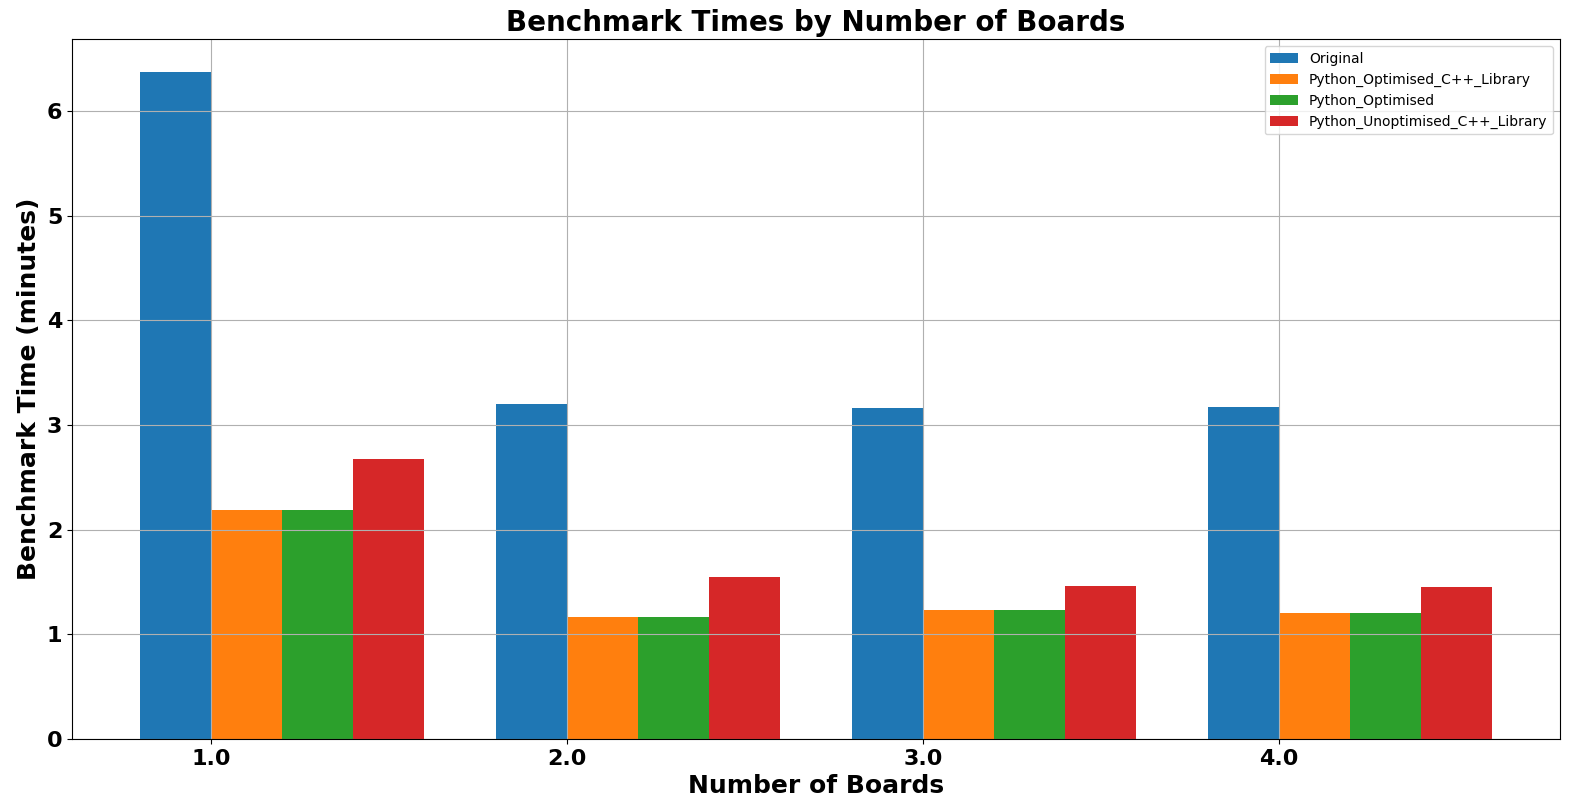
\includegraphics[width=1\textwidth, height=10cm]{~/Documents/Part_D_Modules/Individual_Project/Individual_report/figures/debate_fi.png} % Adjust the path and width as needed
	\caption{Benchmark plot in minutes shown top. Speedup plot shown bottom.}
	\label{fig:debate_fi_plot} % Use this label to reference the figure
\end{figure}

The \texttt{Python\_Unoptimised\_C++\_library} solution achieved a 55\% reduction in runtime, reducing it to 1.45 minutes from 3.17 minutes. However, it resulted in a lower speedup compared to the original, likely due to the limited runtime achieved using only one board. Conversely, the \texttt{Python\_Optimised} solution delivered the most substantial reduction in runtime of 62\% (1.20 minutes compared to 3.17 minutes). Despite this, it also exhibited a lower speedup, which began to degrade after the incorporation of 2 boards. These results were derived from only 5 test scenarios to mitigate the prolonged runtime of the application. The findings indicate that the \texttt{Python\_Optimised} solution reached a plateau, showing no further improvements beyond the use of 2 boards. This plateau may be attributed to the limited runtime where adding additional boards did not yield performance gains, suggesting that the optimal performance with this improved solution can be achieved using only 2 boards instead of 4.

Surprisingly, no significant performance improvement was observed with the \texttt{\seqsplit{Python\_Optimised\_C++\_library}} solution. Given previous results, one might expect that integrating the \texttt{C++} library into the application would enhance performance, and that optimising the multiprocessing design would further boost efficiency. Combining the two was anticipated to yield an even larger performance increase, yet this did not occur. In the \texttt{Python\_Optimised} solution, adding the \texttt{C++} library did not enhance performance; in fact, the performance was identical to when the \texttt{C++} library was not included. This outcome raises an intriguing question: why did only the original \texttt{DeBaTE-FI} platform benefit from integrating the \texttt{C++} library, while no performance gain was observed when the \texttt{C++} library was incorporated into the \texttt{Python\_Optimised} solution? Investigating this discrepancy will be crucial for future efforts to further optimise the software.

All three developed solutions significantly improved the performance of the \texttt{DeBaTE-FI} platform. The \texttt{Python\_Optimised} solution is particularly convenient as it eliminates the need to compile the \texttt{C++} code into a shared library (\texttt{.so}) file. The \texttt{C++} class can be used in the application as the standard \texttt{telnet} library, replacing the older \texttt{Telnetlib} \texttt{Python} library which was deprecated in \texttt{Python 3.11} and is slated for removal in version \texttt{3.13}\cite{PythonTelnetlib}. Additionally, the \texttt{C++} library facilitates the creation of custom functions and allows for prioritization of performance. Therefore, this project proposes the use of the newly developed \texttt{C++} library (\texttt{Telnetlibcpp}) when the \texttt{DeBaTE-FI} platform's code is updated to accommodate later versions of \texttt{Python}.

Results from the main setup (Figure~\ref{fig:debate_fi_setup}) using the \texttt{Python\_Optimised} solution are presented in Table~\ref{tab:debate_metrics}. A 43.5\% performance gain was observed, compared to the 62.1\% improvement noted in the local setup. This still represents a significant enhancement in performance. To further investigate the proposed solution, it would be beneficial to analyse results using a varying number of boards and their respective speed-ups in the main setup. This analysis could help determine the ideal number of boards for optimal performance. Additionally, no results were collected using single-board computers (SBCs) like the Raspberry Pi, primarily due to the time constraints of this project. Investigating the performance of the proposed solution on SBCs could be another valuable area of exploration.

\begin{table}[H]
	\centering
	\begin{tabular}{@{}lcc@{}} % 'l' for left-aligned text, 'c' for centered text
		\toprule
		\textbf{Metric} & \textbf{Local setup} & \textbf{Main setup} \\
		\midrule
		\texttt{STM32} Test Boards & 4 & 36 \\ \hline
		Test scenarios & 5 & 1000 \\ \hline
		Original solution run time(min) & 3.17 & 234.47 \\ \hline
		Optimised solution run time(min) & 1.20 & 132.4 \\ \hline
		Performance improvement(\%) & 62.1 & 43.5 \\ 
		\bottomrule
	\end{tabular}
	\caption{Comparison of benchmark metrics on the local versus the main setup(Figure~\ref{fig:debate_fi_setup}).}
	\label{tab:debate_metrics}
\end{table}